% Created 2017-09-22 Fri 10:51
\documentclass{ximera}
\newcommand{\RR}{\mathbb R}
\renewcommand{\d}{\,d}
\newcommand{\dd}[2][]{\frac{d #1}{d #2}}
\renewcommand{\l}{\ell}
\newcommand{\ddx}{\frac{d}{dx}}
\newcommand{\dfn}{\textbf}
\newcommand{\eval}[1]{\bigg[ #1 \bigg]}

\author{Jim Fowler and Bart Snapp}
\date{\today}
\title{A table of values}
\hypersetup{
  pdfkeywords={},
  pdfsubject={},
  pdfcreator={Emacs 25.2.1 (Org mode 8.2.10)}}
\begin{document}

\begin{abstract}
Given a table of values, find approximations.
\end{abstract}

Let $F:\R^2\to\R$ be a differentiable function that is roughly
described by the following table of values.

\begin{center}
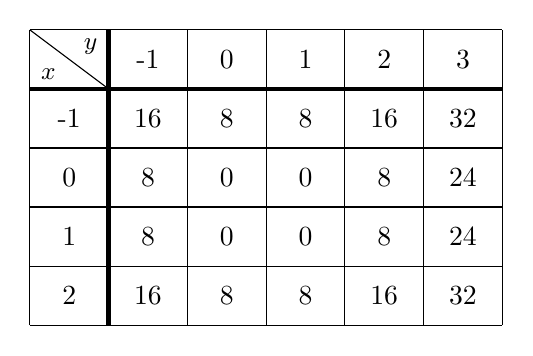
\begin{tikzpicture}[x=1cm,y=.75cm]
  \draw (0,0) grid [step=1] (6,5);
  
  \draw[ultra thick] (0,4)--(6,4);
  \draw[ultra thick] (1,0)--(1,5);
  
  \draw (0,5) -- (1,4);
  \node at (.9,4.9) [below left,inner sep=1pt] {\small$y$};
  \node at (0.1,4.1) [above right,inner sep=1pt] {\small$x$};
  
  %% x-values
  \node at (0.5,3.5) { -1 };
  \node at (0.5,2.5) { 0 };
  \node at (0.5,1.5) { 1 };
  \node at (0.5,0.5) { 2 };
  
  %% y-values
  \node at (1.5,4.5) { -1 };
  \node at (2.5,4.5) { 0 };
  \node at (3.5,4.5) { 1 };
  \node at (4.5,4.5) { 2 };
  \node at (5.5,4.5) { 3 };
  
  %% z-values
  %% top row
  \node at (1.5,3.5) {16};
  \node at (2.5,3.5) {8};
  \node at (3.5,3.5) {8};
  \node at (4.5,3.5) {16};
  \node at (5.5,3.5) {32};
  
  %% second row
  \node at (1.5,2.5) {8};
  \node at (2.5,2.5) {0};
  \node at (3.5,2.5) {0};
  \node at (4.5,2.5) {8};
  \node at (5.5,2.5) {24};
  
  %% third row
  \node at (1.5,1.5) {8};
  \node at (2.5,1.5) {0};
  \node at (3.5,1.5) {0};
  \node at (4.5,1.5) {8};
  \node at (5.5,1.5) {24};
  
  %% bottom row
  \node at (1.5,.5) {16};
  \node at (2.5,.5) {8};
  \node at (3.5,.5) {8};
  \node at (4.5,.5) {16};
  \node at (5.5,.5) {32};
\end{tikzpicture}
\end{center}

\begin{exercise}
What is the value of $F(1,2)$?
\begin{prompt}
\[
  F(1,2) = \answer{8}
\]
\end{prompt}
\end{exercise}

\begin{exercise}
Estimate $F^{(1,0)}(1,2)$ as we did in the textbook.
\begin{prompt}
\[
  F^{(1,0)}(1,2) = \answer{4}
\]
\end{prompt}
\end{exercise}

\begin{exercise}
Estimate $F^{(0,1)}(1,2)$ as we did in the textbook.
\begin{prompt}
\[
  F^{(0,1)}(1,2) = \answer{12}
\]
\end{prompt}
\end{exercise}

\begin{exercise}
Let $z = F(x,y)$ and compute $\d z$ at the point $(1,2)$ in terms of
$\d x$ and $\d y$. This means $\d x $ and $\d y$ will be in your
answer.
\begin{prompt}
\[
  \d z = \answer{4 dx + 12 dy}
\]
\end{prompt}
\end{exercise}

\begin{exercise}
Use $\d z$ to estimate $F(1.5,2.5)$. 
\begin{prompt}
\[
  F(1.5,2.5) \approx \answer{8 + 0.5 \cdot 4 + 0.5 \cdot 12}.
\]
\end{prompt}
\end{exercise}

\begin{exercise}
Find an equation for a tangent plane for $F(x,y)$ at the point $(1,2)$.
\begin{prompt}
\[
z = \answer{(x - 1) \cdot 4 + (y - 2) \cdot 12+8}
\]
\end{prompt}
\end{exercise}

\begin{exercise}
Use your tangent plane to estimate $F(1.5,2.5)$. 
\begin{prompt}
\[
  F(1.5,2.5) \approx \answer{8 + 0.5 \cdot 4 + 0.5 \cdot 12}.
\]
\end{prompt}
\end{exercise}

\begin{exercise}
Estimate the vector $\grad F(1,2)$.
\begin{prompt}
\[
  \grad F(1,2) \approx \vector{\answer{4},\answer{12}}.
\]
\end{prompt}
\end{exercise}
% Emacs 25.2.1 (Org mode 8.2.10)
\end{document}
